\section{Analytic decay}\label{sec:decay}

This section proves the size estimate~(D) of \cref{tab:constants}
(\cref{thm:decay,cor:decay-separated}), which enters the final deduction in
\cref{subsec:main-proof}. Heuristically, $\abs{P^{\alt}_I(\xi_k)}$ is an $n_I$-fold integral whose
integrand is $\exp(-h^2E)$ for a discrete logarithmic energy $E$ of free points interacting with
the nodes and with a confining field $2\pi\abs{\operatorname{Im}z}$ coming from the reflection
formula, so its size is governed by the minimum of a constrained energy problem. Testing that
minimum against an explicit trial measure gives a rigorous lower bound for the decay rate.

\begin{theorem}\label{thm:decay}
For $k\in\{1,2,3,4\}$,
\[
  \limsup_{h\to\infty}\ \frac1{h^2}\max_{I\subseteq\Com,\ \abs I\le1}\log\abs{P^{\alt}_I(\xi_k)}
  \le-\cD_{\alt},\qquad \cD_{\alt}=3.5101772 .
\]
\end{theorem}

The constant $\cD_{\alt}$ is defined to be this decimal number. It is the truncation to seven
decimals of the certified rational lower bound $\cD^{*}_{\alt}=3.5101772515\ldots$ of
\cref{prop:energy-certificate}; it is a lower bound for the true decay rate and is not claimed
to be equal to it.

\begin{corollary}\label{cor:decay-separated}
Put $\cD_{\sep}=\cD_{\alt}+\frac{\log2}{256}$. For $k\in\{1,2,3,4\}$,
\[
  \limsup_{h\to\infty}\ \frac1{h^2}\max_{\abs I\le1}\log\abs{P^{\sep}_I(\xi_k)}\le-\cD_{\sep}
  \le-3.5128848 .
\]
\end{corollary}

\begin{proof}
By \cref{cor:separation},
$\log\abs{P^{\sep}_I(\xi_k)}=\log\abs{P^{\alt}_I(\xi_k)}-m(m-1)\log2$ and
$m(m-1)=h^2/256-h/16$. Finally $(\log2)/256=0.00270760617\ldots\ge0.0027076$ and
$3.5101772+0.0027076=3.5128848$.
\end{proof}

The proof of \cref{thm:decay} has three parts: a representation of the L\"owner entries as
integrals against a measure supported on a contour in the left half-plane and on the poles of $F$
between the contour and the origin (\cref{subsec:contour}); the resulting bound for the
determinant as a multiple integral (\cref{subsec:andreief-bound}); and a comparison of that
integrand with an explicit trial measure by logarithmic potential theory
(\cref{subsec:energy-criterion}). The numerical input is \cref{prop:energy-certificate}. This is
the energy method of~\cite[\S6]{Litsey2026Lowner} (going back to~\cite{OpenAICatalan2026}), in
the weaker form needed for irrationality: we need decay at the single point $\xi_k$, not on a
neighbourhood. Throughout, $\nu$ denotes the limiting node measure
\begin{equation}\label{eq:nu-def}
  \nu=\mathrm{Leb}|_{[0,1]}+\tfrac12\,\mathrm{Leb}|_{[1,1+c]},\qquad \nu(\C)=\lambda=\tfrac{17}{16}.
\end{equation}
For the alternating geometry both $\frac1h\sum_{x\in\Row^{\alt}}\delta_{x/h}$ and
$\frac1h\sum_{y\in\Col^{\alt}}\delta_{y/h}$ converge to $\nu$. We carry out the analysis for the
alternating determinant and transfer it to the separated one by the exact identity of
\cref{cor:separation}; \cref{rem:separated-energy} explains how the same gain appears if the
separated determinant is treated directly.

\subsection{Reflection and a contour representation}\label{subsec:contour}

Let $\Gamma\subset\{\operatorname{Re}z<0\}$ be the contour of \cref{sec:contour-and-measure}
(\cref{fig:contour}): the polygonal path through the vertices $v_0=-r_0,v_1,\dots,v_7$ of
\cref{tab:vertices}, followed by the upward vertical ray from $v_7$, together with its complex
conjugate. Here $r_0=0.1329814$, the ordinates of $v_0,\dots,v_7$ increase, and $\Gamma$ meets
$\R$ only at $-r_0$.

For each $h$ let $x_h$ be the unique number in $(-hr_0-\frac12,-hr_0+\frac12]$ with
$x_h\equiv\frac1{20}\pmod1$, and $\Gamma_h=h\Gamma+(x_h+hr_0)$, the horizontal translate of
$h\Gamma$ crossing $\R$ at $x_h$. We orient $\Gamma_h$ downwards, from $+i\infty$ to $-i\infty$,
so that the nodes lie on its left. Let
\[
  \Atoms_h=\{-s-a:a\in\Z_{\ge0},\ -s-a>x_h\},\qquad
  \Atoms_h'=\{-\tfrac12-a:a\in\Z_{\ge0},\ -\tfrac12-a>x_h\}
\]
be the poles of $F$ between $\Gamma_h$ and $0$, and put
\[
  \mathcal E(z)=\pi\bigl(\cot\pi(z+\tfrac12)-\cot\pi(z+s)\bigr).
\]

\begin{lemma}\label{lem:contour}
For all nodes $x,y\in\Nod$, with $F[x,y]$ as in~\eqref{eq:divided-difference},
\[
  F[x,y]=\int\frac{\dd\Omega_h(z)}{(z-x)(z-y)},\qquad
  \Omega_h=\frac{\mathcal E(z)\,\dd z}{2\pi i}\Big|_{\Gamma_h}
           +\sum_{\rho\in\Atoms_h}\delta_\rho-\sum_{\rho\in\Atoms'_h}\delta_\rho .
\]
Moreover there is $C_1=C_1(k)$, independent of $h$, with
$\abs{\mathcal E(z)}\le C_1\e^{-2\pi\abs{\operatorname{Im}z}}$ for all $z\in\Gamma_h$.
\end{lemma}

\begin{proof}
Fix $x,y$ and let $\phi(z)=F(z)/((z-x)(z-y))$. Its residues at the nodes add up to $F[x,y]$, and
its residue at a pole $\rho$ of $F$ is $\Res_\rho F/((\rho-x)(\rho-y))$, with $\Res_\rho F=-1$ on
$-s-\Z_{\ge0}$ and $+1$ on $-\frac12-\Z_{\ge0}$. Apply the residue theorem to the part of the
region to the right of $\Gamma_h$ inside $\abs z<R$. On the arc $\abs z=R$ joining the two vertical
rays of $\Gamma_h$ we have $\abs{\arg z}\le\frac\pi2+o(1)$, so $F(z)=O(1/R)$ by Stirling's
expansion $\psi(z)=\log z-\frac1{2z}+O(\abs z^{-2})$, uniform in $\abs{\arg z}\le\pi-\delta$
\cite[5.11.2]{DLMF}, and the arc contributes $O(R^{-2})\to0$. Hence
\[
  F[x,y]=\frac1{2\pi i}\int_{\Gamma_h}\phi(z)\,\dd z
  +\sum_{\rho\in\Atoms_h}\frac1{(\rho-x)(\rho-y)}-\sum_{\rho\in\Atoms'_h}\frac1{(\rho-x)(\rho-y)} .
\]
On $\Gamma_h$ we split $F=G+\mathcal E$ with $G(z)=\psi(1-z-s)-\psi(1-z-\frac12)$, using the
reflection formula $\psi(w)=\psi(1-w)-\pi\cot\pi w$ \cite[5.5.4]{DLMF}. The poles of $G$ lie at
$1-s+a$ and $\frac12+a$ ($a\ge0$), so $G$ is holomorphic on $\operatorname{Re}z<\frac15$; for
$\operatorname{Re}z\le0$ both arguments $1-z-s$ and $1-z-\frac12$ have real part at least
$\frac15$, and Stirling's expansion gives $G(z)=(s-\frac12)/z+O(\abs z^{-2})$. The region to the
left of $\Gamma_h$ lies in $\operatorname{Re}z<0$, so $G(z)/((z-x)(z-y))$ is holomorphic there
and $O(\abs z^{-3})$; closing the contour to the left shows that its integral over $\Gamma_h$
vanishes. This proves the representation.

For the bound, write $w=z+s$ or $z+\frac12$ and $\upsilon=\operatorname{Im}w=\operatorname{Im}z$.
For $\upsilon>0$ one has $\cot\pi w+i=2i\e^{2\pi iw}/(\e^{2\pi iw}-1)$, so
$\abs{\cot\pi w+i}\le2\e^{-2\pi\upsilon}/(1-\e^{-2\pi\upsilon})$; similarly for $\upsilon<0$ with
$-i$. Since $\mathcal E(z)$ is $\pi$ times the difference of the two values of $\cot\pi w\pm i$,
\[
  \abs{\mathcal E(z)}\le\frac{4\pi}{1-\e^{-2\pi\eta}}\,\e^{-2\pi\abs{\operatorname{Im}z}}
  \qquad\text{when }\abs{\operatorname{Im}z}\ge\eta,
\]
for any $\eta>0$. Take $\eta=\frac1{10}$. The first edge of $\Gamma$ goes from $v_0$ to
$v_1=v_0+(-0.0218611+0.04\,i)$ (\cref{tab:vertices}), and $h\cdot0.04>\eta$, so the part of
$\Gamma_h$ with $\abs{\operatorname{Im}z}<\eta$ lies on the two edges through $x_h$, and its points
satisfy $\abs{\operatorname{Re}z-x_h}<\frac{0.0218611}{0.04}\,\eta<0.055$. The poles of $\mathcal E$
are the points of $-s+\Z$ and $-\frac12+\Z$; their fractional parts belong to
$\{\frac15,\frac25,\frac35,\frac45,\frac12\}$, so they are at distance at least $\frac3{20}$ from
$x_h\equiv\frac1{20}\pmod1$. Hence that part of $\Gamma_h$ lies in the set of $z$ with
$\abs{\operatorname{Im}z}\le\frac1{10}$ at distance at least $\frac3{20}-0.055>0.09$ from every pole
of $\mathcal E$. This set is invariant under $z\mapsto z+1$ and compact modulo this translation,
and $\mathcal E$ is continuous and $1$-periodic on it, hence bounded there by a constant $B(k)$
independent of $h$. The lemma holds with $C_1=\max\bigl(4\pi/(1-\e^{-\pi/5}),\,B(k)\e^{\pi/5}\bigr)$.
\end{proof}

\subsection{The Andr\'eief bound}\label{subsec:andreief-bound}

Let $S_h=\Gamma_h\cup\Atoms_h\cup\Atoms'_h$. It lies at distance at least $\frac15$ from $\Nod$
(the nearest pole to $0$ is $-s$ or $-\frac12$), and $\abs{\Omega_h}$ is a finite measure on it
by \cref{lem:contour}.

\begin{lemma}\label{lem:andreief-bound}
For $\abs I\le1$, with $\Row=\Row^{\alt}_I$, $\Col=\Col^{\alt}_I$ and $n'=n_I$,
\[
  \abs{P^{\alt}_I(\xi_k)}\le\frac{\Delta(\Row)\Delta(\Col)}{n'!}\int_{S_h^{n'}}
  \abs{\Delta(z)}^2\prod_{c=1}^{n'}\frac1{\abs{\omega_\Row(z_c)\,\omega_\Col(z_c)}}\,
  \dd\abs{\Omega_h}^{\otimes n'}(z).
\]
The integrand vanishes unless the $z_c$ are pairwise distinct.
\end{lemma}

\begin{proof}
By \cref{lem:contour}, $M^{\alt}_I(\xi_k)$ is the matrix of \cref{prop:det-formula} for the
measure $\Omega_h$ on $S_h$. Take absolute values. The last assertion is clear from
$\Delta(z)^2$.
\end{proof}

\subsection{Logarithmic energy}\label{subsec:energy-prelim}

For finite signed Borel measures $\mu_1,\mu_2$ with compact support put
$\pot{\mu_1}(z)=\int-\log\abs{z-w}\,\dd\mu_1(w)$,
$I(\mu_1,\mu_2)=\iint-\log\abs{z-w}\,\dd\mu_1\dd\mu_2$ and $I(\mu_1)=I(\mu_1,\mu_1)$, whenever
these are absolutely convergent. For a finite family of points $(\zeta_c)$ with weights $1/h$,
$\sigma=\frac1h\sum_c\delta_{\zeta_c}$, we use the energy without diagonal
$I^*(\sigma)=h^{-2}\sum_{c\ne c'}-\log\abs{\zeta_c-\zeta_{c'}}$.

\begin{lemma}[Conditional positivity]\label{lem:cond-pos}
Let $\eta$ be a signed measure with compact support, $\eta(\C)=0$ and
$\iint\abs{\log\abs{z-w}}\,\dd\abs\eta(z)\,\dd\abs\eta(w)<\infty$. Then $I(\eta)\ge0$.
\end{lemma}

\begin{proof}
This is classical (see~\cite{SaffTotik1997}); we include the short argument. For $x\ne0$,
Frullani's integral gives $-\log\abs x=\frac12\int_0^\infty(\e^{-t\abs x^2}-\e^{-t})\,\frac{\dd t}t$,
and the integrand has constant sign for fixed $x$, so
$\int_0^\infty\abs{\e^{-t\abs x^2}-\e^{-t}}\frac{\dd t}t=2\abs{\log\abs x}$. By the hypothesis
Fubini's theorem applies, and since $\eta(\C)=0$ the term $\e^{-t}$ integrates to zero:
\[
  I(\eta)=\frac12\int_0^\infty\Bigl(\iint\e^{-t\abs{z-w}^2}\,\dd\eta(z)\,\dd\eta(w)\Bigr)\frac{\dd t}t .
\]
The inner integral equals $\frac1{4\pi t}\int_{\R^2}\e^{-\abs\xi^2/(4t)}\abs{\hat\eta(\xi)}^2\,\dd\xi\ge0$,
where $\hat\eta(\xi)=\int\e^{i\langle\xi,z\rangle}\dd\eta(z)$, because the Gaussian
$\e^{-t\abs x^2}$ is the Fourier transform of the positive function
$\frac1{4\pi t}\e^{-\abs\xi^2/(4t)}$.
\end{proof}

All measures to which we apply \cref{lem:cond-pos} are differences of finitely many measures
with bounded densities on segments, on intervals or on circles; they satisfy its hypothesis.

\begin{lemma}[Circles]\label{lem:circles}
Let $\sigma_{a,r}$ be the normalized arclength measure on the circle $\abs{z-a}=r$. Then
$\pot{\sigma_{a,r}}(z)=-\log\max(\abs{z-a},r)$. Consequently $I(\sigma_{a,r})=-\log r$ and
$I(\sigma_{a,r},\sigma_{b,r})\le-\log\abs{a-b}$ for $a\ne b$.
\end{lemma}

\begin{proof}
The formula for the potential is Gauss's mean value property of $\log\abs{z-w}$ for
$\abs{z-a}>r$, and Jensen's formula for $\abs{z-a}\le r$. Since $-\log\max(t,r)\le-\log t$,
integrating $\pot{\sigma_{b,r}}\le-\log\abs{\cdot-b}$ against $\sigma_{a,r}$ gives
$I(\sigma_{a,r},\sigma_{b,r})\le\pot{\sigma_{a,r}}(b)\le-\log\abs{a-b}$.
\end{proof}

We call a measure \emph{segment-regular} if it is a finite sum of measures with bounded density
with respect to arclength on line segments. The potential of a segment-regular measure is
uniformly continuous on the whole plane, with a modulus of continuity $O(\delta\log(1/\delta))$
(\cref{lem:uniform-continuity}); we use this at points that range over unbounded sets. The
measure $\nu$ is segment-regular, and $I(\nu)$ is computed in closed form in \cref{lem:Inu}.

\subsection{The energy criterion}\label{subsec:energy-criterion}

\begin{proposition}[Energy criterion]\label{prop:energy-criterion}
Let $\mu$ be a positive segment-regular measure of mass $\lambda$, supported in
$(\Gamma\cup[-r_0,0])\cap\{\abs z\le1\}$. (The proof uses only that $\mu$ is segment-regular, of
mass $\lambda$ and supported in $\{\abs z\le1\}$; positivity and the location of the support are
natural for the extremal problem of \cref{rem:energy-meaning} and are satisfied by the trial
measure.) Let $0<\varepsilon_0<1$ and
\[
  V(z)=\pot\mu(z)-\pot\nu(z)+(1-\varepsilon_0)\pi\abs{\operatorname{Im}z}.
\]
Suppose that $\theta\in\R$ satisfies $V(z)>\theta$ for all $z\in\Gamma$, and put
$J=\int_{-r_0}^0\min\bigl(V(t)-\theta,0\bigr)\,\dd t$. Then for every $k$,
\[
  \limsup_{h\to\infty}\ \frac1{h^2}\max_{\abs I\le1}\log\abs{P^{\alt}_I(\xi_k)}
  \le-\bigl(2\lambda\theta+4J-I(\mu)+I(\nu)\bigr).
\]
\end{proposition}

\begin{proof}
All $o(1)$ terms below tend to $0$ as $h\to\infty$, uniformly in $\abs I\le1$ and in the
configuration $z\in S_h^{n'}$. By \cref{lem:uniform-continuity}, $\pot\mu$ and $\pot\nu$ are
uniformly continuous on $\C$, and $\abs{\operatorname{Im}z}$ is $1$-Lipschitz; so $V$ is uniformly
continuous on $\C$, with a modulus of continuity that we denote by $\omega_V$. Moreover
$\pot\mu-\pot\nu$ tends to $0$ at infinity, because the two measures have the same mass and
compact supports; so $V(z)\to+\infty$ along the vertical rays of $\Gamma$, and as $V>\theta$ on
$\Gamma$ and $V$ is continuous, there is $\eta_0>0$ with $V\ge\theta+\eta_0$ on $\Gamma$.

\emph{Step 1: scaling.} Put $\zeta_c=z_c/h$, $\sigma=\frac1h\sum_c\delta_{\zeta_c}$,
$\nu_\Row=\frac1h\sum_{x\in\Row}\delta_{x/h}$, $\nu_\Col$ likewise and
$\bar\nu_h=\frac12(\nu_\Row+\nu_\Col)$, of mass $n'/h$. Counting the factors $h$ in each product,
\begin{equation}\label{eq:scaled-integrand}
  \log\frac{\Delta(\Row)\Delta(\Col)\abs{\Delta(z)}^2}{\prod_c\abs{\omega_\Row(z_c)\omega_\Col(z_c)}}
  =-2n'\log h+h^2\Bigl[-\tfrac12I^*(\nu_\Row)-\tfrac12I^*(\nu_\Col)-I^*(\sigma)
  +2I(\sigma,\bar\nu_h)\Bigr].
\end{equation}

\emph{Step 2: the nodes.} We claim $\frac12(I^*(\nu_\Row)+I^*(\nu_\Col))\ge I(\nu)-o(1)$. Replace each
node $x$ by the uniform measure $\varsigma_x$ of mass $1/h$ on $[x/h,(x+1)/h]$, and let
$\lambda_\Row=\sum_{x\in\Row}\varsigma_x$, $\lambda_\Col$ likewise. For nodes with $\abs{x-x'}=j\ge2$,
$I(\varsigma_x,\varsigma_{x'})\le h^{-2}(-\log(j/h)+2/j)$, and for $j=1$ the excess over
$-h^{-2}\log(1/h)$ is at most $\frac32h^{-2}$; the self-energies are
$I(\varsigma_x)=h^{-2}(\frac32+\log h)$. Summing,
$I(\lambda_\Row)\le I^*(\nu_\Row)+O(h^{-1}\log h)$, and likewise for $\Col$. By the parallelogram
identity and \cref{lem:cond-pos},
\[
  \tfrac12\bigl(I(\lambda_\Row)+I(\lambda_\Col)\bigr)
  =I\bigl(\tfrac12(\lambda_\Row+\lambda_\Col)\bigr)+\tfrac14I(\lambda_\Row-\lambda_\Col)
  \ge I\bigl(\tfrac12(\lambda_\Row+\lambda_\Col)\bigr).
\]
In either geometry every border cell belongs to exactly one of $\Row,\Col$, so
$\frac12(\lambda_\Row+\lambda_\Col)=\nu-\varsigma_I$, where $\varsigma_I$ is the cell of the deleted
node ($\varsigma_\varnothing=0$). Finally $I(\nu-\varsigma_I)\ge I(\nu)-2\sup\pot\nu/h=I(\nu)-O(1/h)$.

\emph{Step 3: the free points.} We claim that for every configuration with distinct points,
\[
  I^*(\sigma)\ge2\int\pot{\mu_h}\,\dd\sigma-I(\mu_h)-o(1),\qquad\mu_h=\frac{n'}{\lambda h}\,\mu .
\]
Let $\sigma'=\frac1h\sum_c\sigma_{\zeta_c,h^{-2}}$ (\cref{lem:circles}). By \cref{lem:circles},
$I(\sigma')\le I^*(\sigma)+n'h^{-2}\cdot2\log h=I^*(\sigma)+o(1)$. The measure $\sigma'-\mu_h$ has
compact support, total mass $0$ and finite energy, so \cref{lem:cond-pos} gives
$I(\sigma')\ge2I(\sigma',\mu_h)-I(\mu_h)$. Finally
$I(\sigma',\mu_h)=\frac1h\sum_c\int\pot{\mu_h}\dd\sigma_{\zeta_c,h^{-2}}\ge\int\pot{\mu_h}\dd\sigma-o(1)$:
the points $\zeta_c$ range over the unbounded set $S_h/h$, but by \cref{lem:uniform-continuity}
the potential $\pot\mu$ has a modulus of continuity $\omega$ valid on all of $\C$, so each of the
$n'$ terms changes by at most $\frac{n'}{\lambda h}\,\omega(h^{-2})$ when the circle of radius
$h^{-2}$ is replaced by its centre, uniformly in the configuration.

\emph{Step 4: replacing the discrete node measure.} We claim
$\abs{(\pot{\mu_h}-\pot{\bar\nu_h})(\zeta)-(\pot\mu-\pot\nu)(\zeta)}=o(1)$ uniformly for
$\zeta\in S_h/h$. For $\abs\zeta\ge4$, the measures $\mu_h-\bar\nu_h$ and $\mu-\nu$ both have mass
zero and support in $\{\abs w\le2\}$, so both potentials are integrals of
$k_\zeta(w)=-\log\abs{1-w/\zeta}$, which is bounded by $\log2$ and $\frac12$-Lipschitz in $w$
there. Now $\abs{\mu_h-\mu}(\C)=O(1/h)$; $\bar\nu_h$ and $\frac12(\lambda_\Row+\lambda_\Col)$ differ
by moving mass $1/h$ by at most $1/h$; and $\frac12(\lambda_\Row+\lambda_\Col)=\nu-\varsigma_I$. So the
difference is $O(1/h)$. For $\abs\zeta\le4$, $\pot{\mu_h}-\pot\mu=O(1/h)$; and since every point of
$S_h$ is at distance at least $\frac15$ from every cell $[x,x+1]$, $x\in\Nod$ (the atoms are at
most $-\frac15$, and the contour $\Gamma_h$ lies in $\operatorname{Re}z\le x_h<-1$),
$\abs{\pot{\bar\nu_h}(\zeta)-\pot{\nu-\varsigma_I}(\zeta)}\le\frac1h\sum_{x}1/\mathrm{dist}(h\zeta,[x,x+1])
=O(h^{-1}\log h)$, while $\pot{\varsigma_I}(\zeta)=O(h^{-1}\log h)$.

\emph{Step 5: the weights.} By \cref{lem:contour}, on $\Gamma_h$ we have
$\dd\abs{\Omega_h}(z)\le\frac{C_1}{2\pi}\e^{-2\pi\abs{\operatorname{Im}z}}\abs{\dd z}
=\frac{C_1}{2\pi}\e^{-2\pi(1-\varepsilon_0)h\abs{\operatorname{Im}\zeta}}\,\dd\varkappa_h(z)$,
where $\varkappa_h$ denotes the measure $\e^{-2\pi\varepsilon_0\abs{\operatorname{Im}z}}\abs{\dd z}$
on $\Gamma_h$ plus unit masses at the atoms. Its total mass is $O(h)$: the finite part of $\Gamma_h$
has length $O(h)$, the two rays contribute $1/(\pi\varepsilon_0)$, and there are $O(h)$ atoms.

\emph{Step 6: assembling.} Insert Steps 2--5 into~\eqref{eq:scaled-integrand}, drop
$-2n'\log h\le0$ and use $I(\mu_h)=I(\mu)+O(1/h)$. Since $n'=O(h)$, the integrand of
\cref{lem:andreief-bound} is at most
\[
  \exp\Bigl(h^2\bigl[I(\mu)-I(\nu)+o(1)\bigr]-2h\sum_cV(\zeta_c)\Bigr)\,
  \Bigl(\tfrac{C_1}{2\pi}+1\Bigr)^{n'}\dd\varkappa_h^{\otimes n'}(z).
\]

\emph{Step 7: the potential sum.} The free points on $\Gamma_h$ satisfy
$\zeta_c\in\Gamma+(x_h+hr_0)/h$, a translate of $\Gamma$ by at most $1/(2h)$, so
$V(\zeta_c)\ge\theta+\eta_0-\omega_V(1/(2h))\ge\theta$ for large $h$, by the uniform continuity of
$V$ on $\C$ (the points on the vertical rays are unbounded). The free points at atoms are distinct
elements of $(\Atoms_h\cup\Atoms'_h)/h$, so
\[
  \sum_{c:\,z_c\text{ atom}}V(\zeta_c)\ge\theta\cdot\#\{c:z_c\text{ atom}\}
  +\sum_{\rho\in\Atoms_h\cup\Atoms'_h}\min\bigl(V(\rho/h)-\theta,0\bigr).
\]
Each of $\Atoms_h/h$ and $\Atoms'_h/h$ is a progression of step $1/h$ contained in
$(x_h/h,0)\subset(-r_0-\frac1{2h},0)$, with a point within $1/h$ of each end of this interval.
At most one point of each progression lies to the left of $-r_0$, outside the domain of
integration of $J$; these at most two atoms contribute $O(1)$ to the sum, because
$\min(V-\theta,0)$ is bounded on $[-r_0-1,0]$. The other points of each progression fill
$[-r_0,0)$ with step $1/h$, and $\min(V-\theta,0)$ is uniformly continuous, so each of the two
Riemann sums is $hJ+o(h)$. Hence $\sum_cV(\zeta_c)\ge n'\theta+2hJ-o(h)=h(\lambda\theta+2J)-o(h)$.

\emph{Step 8: integration.} Integrating the bound of Step~6 with the lower bound of Step~7,
\[
  \abs{P^{\alt}_I(\xi_k)}\le\exp\Bigl(h^2\bigl[I(\mu)-I(\nu)-2\lambda\theta-4J+o(1)\bigr]\Bigr)
  \cdot\frac{\bigl((\frac{C_1}{2\pi}+1)\varkappa_h(S_h)\bigr)^{n'}}{n'!}.
\]
The last factor is at most $(O(h)/n')^{n'}\e^{n'}=\e^{O(h)}$, which proves the proposition.
\end{proof}

\begin{remark}\label{rem:energy-meaning}
Heuristically, the decay rate is the minimum of
$I(\sigma-\nu)+2\pi\int\abs{\operatorname{Im}\zeta}\,\dd\sigma(\zeta)$ over measures $\sigma$ of mass
$\lambda$ on $\Gamma\cup[-r_0,0]$ whose density on $[-r_0,0]$ is at most $2$, the density of the
two progressions of atoms. The quantity $2\lambda\theta+4J-I(\mu)+I(\nu)$ is the lower bound for
this minimum that conditional positivity extracts from the trial measure $\mu$, the factor
$1-\varepsilon_0$ being reserved to make the contour integrals converge. The trial measure of
\cref{sec:contour-and-measure} has density $2-O(10^{-9})$ on $[-r_0,0]$: the density constraint
is active there.
\end{remark}

\begin{remark}[The separated geometry seen by energy]\label{rem:separated-energy}
Step~2 of the proof holds verbatim for the separated geometry, but there the term
$\frac14I(\lambda_\Row-\lambda_\Col)$ that we dropped does not tend to zero: it tends to
$\frac14I\bigl(\mathrm{Leb}|_{[1,1+c/2]}-\mathrm{Leb}|_{[1+c/2,1+c]}\bigr)$. For two adjacent
intervals of length $a$ this energy equals $4a^2\log2$ (\cref{subsec:energy-formulas}), so with
$a=c/2$ the term is $\frac{c^2}4\log2=\frac{\log2}{256}$. Treating the separated determinant
directly therefore recovers the gain of \cref{cor:separation} in the limit; the identity is its
exact finite-$h$ form.
\end{remark}

\subsection{The certified constants}\label{subsec:energy-certificate}

\begin{proposition}[Computer-assisted]\label{prop:energy-certificate}
Let $\Gamma$ and $\mu$ be the polygon and the trial measure of \cref{sec:contour-and-measure} and
$\varepsilon_0=10^{-6}$. Then $\mu$ satisfies the hypotheses of \cref{prop:energy-criterion}, and
there are numbers $\theta$, $J_-$ and $U_+$ with $V>\theta$ on $\Gamma$, $J\ge J_-$,
$I(\mu)\le U_+$ and
\[
  \theta=2.1001432662\ldots,\qquad J_-=-0.0598567117\ldots,\qquad U_+=2.3239023213\ldots .
\]
Together with $I(\nu)=\frac{867}{512}+\frac{483}{256}\log2-\frac{81}{64}\log3=1.6107019792\ldots$
(\cref{lem:Inu}), this gives $2\lambda\theta+4J-I(\mu)+I(\nu)\ge3.5101772515\ldots$.
\end{proposition}

\begin{proof}
This is a finite computation in ball arithmetic ($256$ bits) with exact rational geometry,
described in \cref{sec:error-analysis}. The potential $V$ is enclosed at the endpoints of $3639$
cells covering the finite part of $\Gamma^+$, and a bound on its second derivative along each cell
controls the values in between; the vertical rays are handled by a monotonicity argument;
$J$ is bounded below by the same chord estimate on $760$ cells of $[-r_0,0]$; and $I(\mu)$ is a
finite sum of segment pair energies in closed form. Every asserted inequality is checked on ball
endpoints or in exact rational arithmetic.
\end{proof}

\emph{Status.} Certified (AI-internal): this is the computation made in the AI-internal audit. The
original fixed-point verifier, with a coarser cover, gives the slightly weaker bound
$3.5101522752\ldots$; the original archive states the rounded bound $3.5099$.

\begin{proof}[Proof of \cref{thm:decay}]
Combine \cref{prop:energy-criterion,prop:energy-certificate}.
\end{proof}

\begin{figure}[t]
\centering
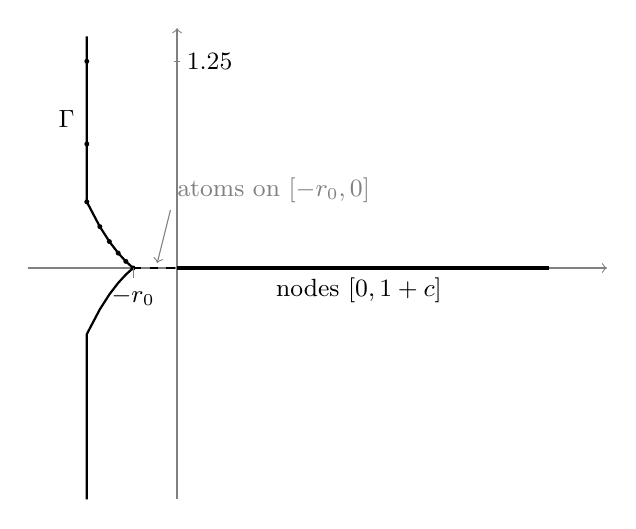
\begin{tikzpicture}[x=4.2cm,y=2.1cm]
  \draw[->,gray] (-0.45,0) -- (1.3,0);
  \draw[->,gray] (0,-1.4) -- (0,1.45);
  \draw[very thick] (0,0) -- (1.125,0);
  \node[below] at (0.55,0) {\small nodes $[0,1+c]$};
  \draw[thick,dashed] (-0.1329814,0) -- (0,0);
  \draw[thick] (-0.1329814,0) -- (-0.1548425,0.04) -- (-0.177904,0.09) -- (-0.2046703,0.16)
     -- (-0.2334108,0.25) -- (-0.2728752,0.4) -- (-0.2728752,0.75) -- (-0.2728752,1.25)
     -- (-0.2728752,1.4);
  \draw[thick] (-0.1329814,0) -- (-0.1548425,-0.04) -- (-0.177904,-0.09) -- (-0.2046703,-0.16)
     -- (-0.2334108,-0.25) -- (-0.2728752,-0.4) -- (-0.2728752,-0.75) -- (-0.2728752,-1.25)
     -- (-0.2728752,-1.4);
  \foreach \p in {(-0.1329814,0),(-0.1548425,0.04),(-0.177904,0.09),(-0.2046703,0.16),
     (-0.2334108,0.25),(-0.2728752,0.4),(-0.2728752,0.75),(-0.2728752,1.25)}
     {\fill \p circle (0.9pt);}
  \node[left] at (-0.28,0.9) {\small $\Gamma$};
  \draw[gray,->] (-0.02,0.35) node[above right=-1pt] {\small atoms on $[-r_0,0]$} -- (-0.06,0.03);
  \draw[gray] (-0.1329814,0) -- (-0.1329814,-0.06);
  \node[below] at (-0.1329814,-0.06) {\small $-r_0$};
  \node[right] at (0,1.25) {\small $1.25$};
  \draw[gray] (-0.01,1.25) -- (0.01,1.25);
\end{tikzpicture}
\caption{The scaled contour $\Gamma$ (vertices $v_0,\dots,v_7$ marked, vertical rays beyond
$v_7$ and $\bar v_7$), the interval $[-r_0,0]$ carrying the scaled poles of $F$, and the node
interval $[0,1+c]$. The horizontal scale is twice the vertical one.}
\label{fig:contour}
\end{figure}
